\documentclass[sigconf,review,anonymous]{acmart}

\usepackage{amsmath}
\usepackage{booktabs}
\usepackage{graphicx}
\usepackage{multirow}
\usepackage{placeins}
\usepackage{xcolor}

\setcopyright{none}
\settopmatter{printacmref=true, printccs=true, printfolios=true}
\renewcommand\footnotetextcopyrightpermission[1]{}
\pagestyle{plain}
\emergencystretch=2em
\acmConference[KDD '27]{ACM SIGKDD Conference on Knowledge Discovery and Data Mining}{2027}{}
\acmBooktitle{Proceedings of the ACM SIGKDD Conference on Knowledge Discovery and Data Mining (KDD '27)}
\acmDOI{}
\acmYear{2027}
\copyrightyear{2027}

\newcommand{\dataset}{\textsc{SiteXRD-Bench}}
\newcommand{\gphase}{$\gamma$}
\newcommand{\gp}{\ensuremath{\gamma^{\prime}}}
\newcommand{\lone}{$\mathrm{L1_2}$}
\title[SiteXRD-Bench]{SiteXRD-Bench: A Hierarchical Benchmark for Chemical-Order Inference and Overlapping-Peak Decomposition in Structural Alloys}

% KDD Datasets and Benchmarks is single blind. Replace this block only with
% verified author metadata before submission; do not invent review identities.
\author{Anonymous Author(s)}
\affiliation{\institution{Anonymous Institution}\country{Anonymous}}

\begin{abstract}
Powder X-ray diffraction (XRD) is a central materials characterization signal,
but it is also a lossy inverse problem: many three-dimensional atomic states can
map to nearly the same one-dimensional pattern. Existing XRD machine-learning
benchmarks largely reward phase labels or whole-pattern reconstruction, leaving
open a harder question: did the model recover the latent physical state that
generated the observation?

We introduce \dataset{}, one benchmark with two independent task tracks for
latent-state recovery from powder XRD. HEA-SRO provides 84,019
quality-controlled high-entropy-alloy structure--XRD pairs with
permutation-invariant first- and second-shell Warren--Cowley short-range order
targets under ID, composition OOD, chemistry OOD, SRO OOD, and matched simulated
perturbations. Gamma-Decomp (gamma/gamma-prime decomposition) provides 10,000
\gphase{}/\gp{} mixture patterns and 21,116 overlap windows with pre-mixing
phase/HKL component truth, peak centers, widths, and areas.

The benchmark exposes both learnable structure and principled non-identifiability.
On ID HEA-SRO, Spectrum Transformer improves SRO MAE over Composition Ridge by
24.4\% (95\% group-bootstrap interval 23.8--24.9\%). On Gamma-Decomp, Peak
Feature improves component F1 over a no-spectrum prior by 0.260 (0.207--0.313)
on full patterns and 0.740 (0.717--0.762) on overlap windows. Yet none of 4,000
same-composition occupancy pairs exceeds the frozen simulated-perturbation
identifiability threshold. Thus \dataset{} evaluates not only accuracy, but also
shortcut use, OOD behavior, component ambiguity, and abstention. Because no
repeated experimental spectra have exact SRO or component truth, v1.1 makes no
claim of experimental-noise calibration or unique occupancy recovery.
\end{abstract}

\begin{CCSXML}
<ccs2012>
 <concept><concept_id>10010147.10010257</concept_id><concept_desc>Computing methodologies~Machine learning</concept_desc><concept_significance>500</concept_significance></concept>
 <concept><concept_id>10002950.10003624</concept_id><concept_desc>Mathematics of computing~Probability and statistics</concept_desc><concept_significance>300</concept_significance></concept>
</ccs2012>
\end{CCSXML}
\ccsdesc[500]{Computing methodologies~Machine learning}
\ccsdesc[300]{Mathematics of computing~Probability and statistics}
\keywords{X-ray diffraction, short-range order, high-entropy alloys,
Ni-based superalloys, inverse problems, out-of-distribution generalization}

\begin{document}
\maketitle

\section{Introduction}

Powder XRD is non-destructive, scalable, and sensitive to long-range crystal
structure, but its inverse problem is underdetermined: a measured
one-dimensional pattern aggregates many reflections and can be compatible with
multiple latent structures. This matters when the target is local chemical
order or phase-resolved components rather than a coarse phase label.

The motivating failure case is concrete. In the public HEA training split, two
Co$_{0.25}$Cr$_{0.25}$Fe$_{0.25}$Ni$_{0.25}$ FCC structures selected by a
frozen rule have XRD cosine similarity 0.9967 but first/second-shell SRO
$L_1$ distance 13.33 (Figure~\ref{fig:hea_sro_example}). A model can fit the
dominant Bragg pattern and still miss the local chemical order. The same
disconnect appears in \gphase{}/\gp{} mixtures: a low residual after summing
peaks does not show whether intensity was assigned to the correct phase/HKL
components. \dataset{} is built around this distinction between looking right
and being physically right.

Two alloy settings expose complementary ambiguities. In high-entropy alloys
(HEAs), structures with the same composition and BCC/FCC parent lattice can
differ in atomic arrangement and short-range order (SRO), while their dominant
Bragg peaks remain similar~\cite{miracle2017hea,george2019hea,zhang2020sro}.
In Ni-based superalloys, FCC \gphase{} and \lone{} \gp{} have related lattices;
their reflections overlap under broadening, strain, and acquisition effects
~\cite{reed2006superalloys,devaux2008gamma,mignanelli2017dual}.

\dataset{} separates observational fit from latent correctness. It contributes
(1) a shared structure--reflection--component--observation hierarchy, (2)
same-composition HEA controls and traceable \gphase{}/\gp{} mixtures, (3)
task-specific permutation-invariant metrics, and (4) grouped ID/OOD protocols,
identifiability diagnostics, and parent-aware uncertainty estimates. Strength
and creep-life prediction are outside the benchmark contract.

\section{Related Work and Positioning}

Rietveld refinement remains the canonical whole-pattern framework
~\cite{rietveld1969}; pseudo-Voigt line shapes provide a standard representation
of diffraction broadening~\cite{thompson1987tch}. A good profile fit, however,
does not prove unique site occupancy. Warren--Cowley coefficients summarize
conditional neighbor probabilities without assigning arbitrary atom indices
~\cite{cowley1950}.

XRD learning has addressed symmetry classification, augmentation, and
multiphase identification or quantification
~\cite{vecsei2019symmetry,oviedo2019xrd,lee2020multiphase,greasley2023multiphase},
while set prediction supports unordered component outputs
~\cite{lee2019settransformer,carion2020detr}. Calibration and domain
generalization motivate controlled shifts rather than random-split accuracy
alone~\cite{guo2017calibration,gulrajani2021domainbed}.

\IfFileExists{generated/dataset_overview.png}{
\begin{figure*}[t]
  \centering
  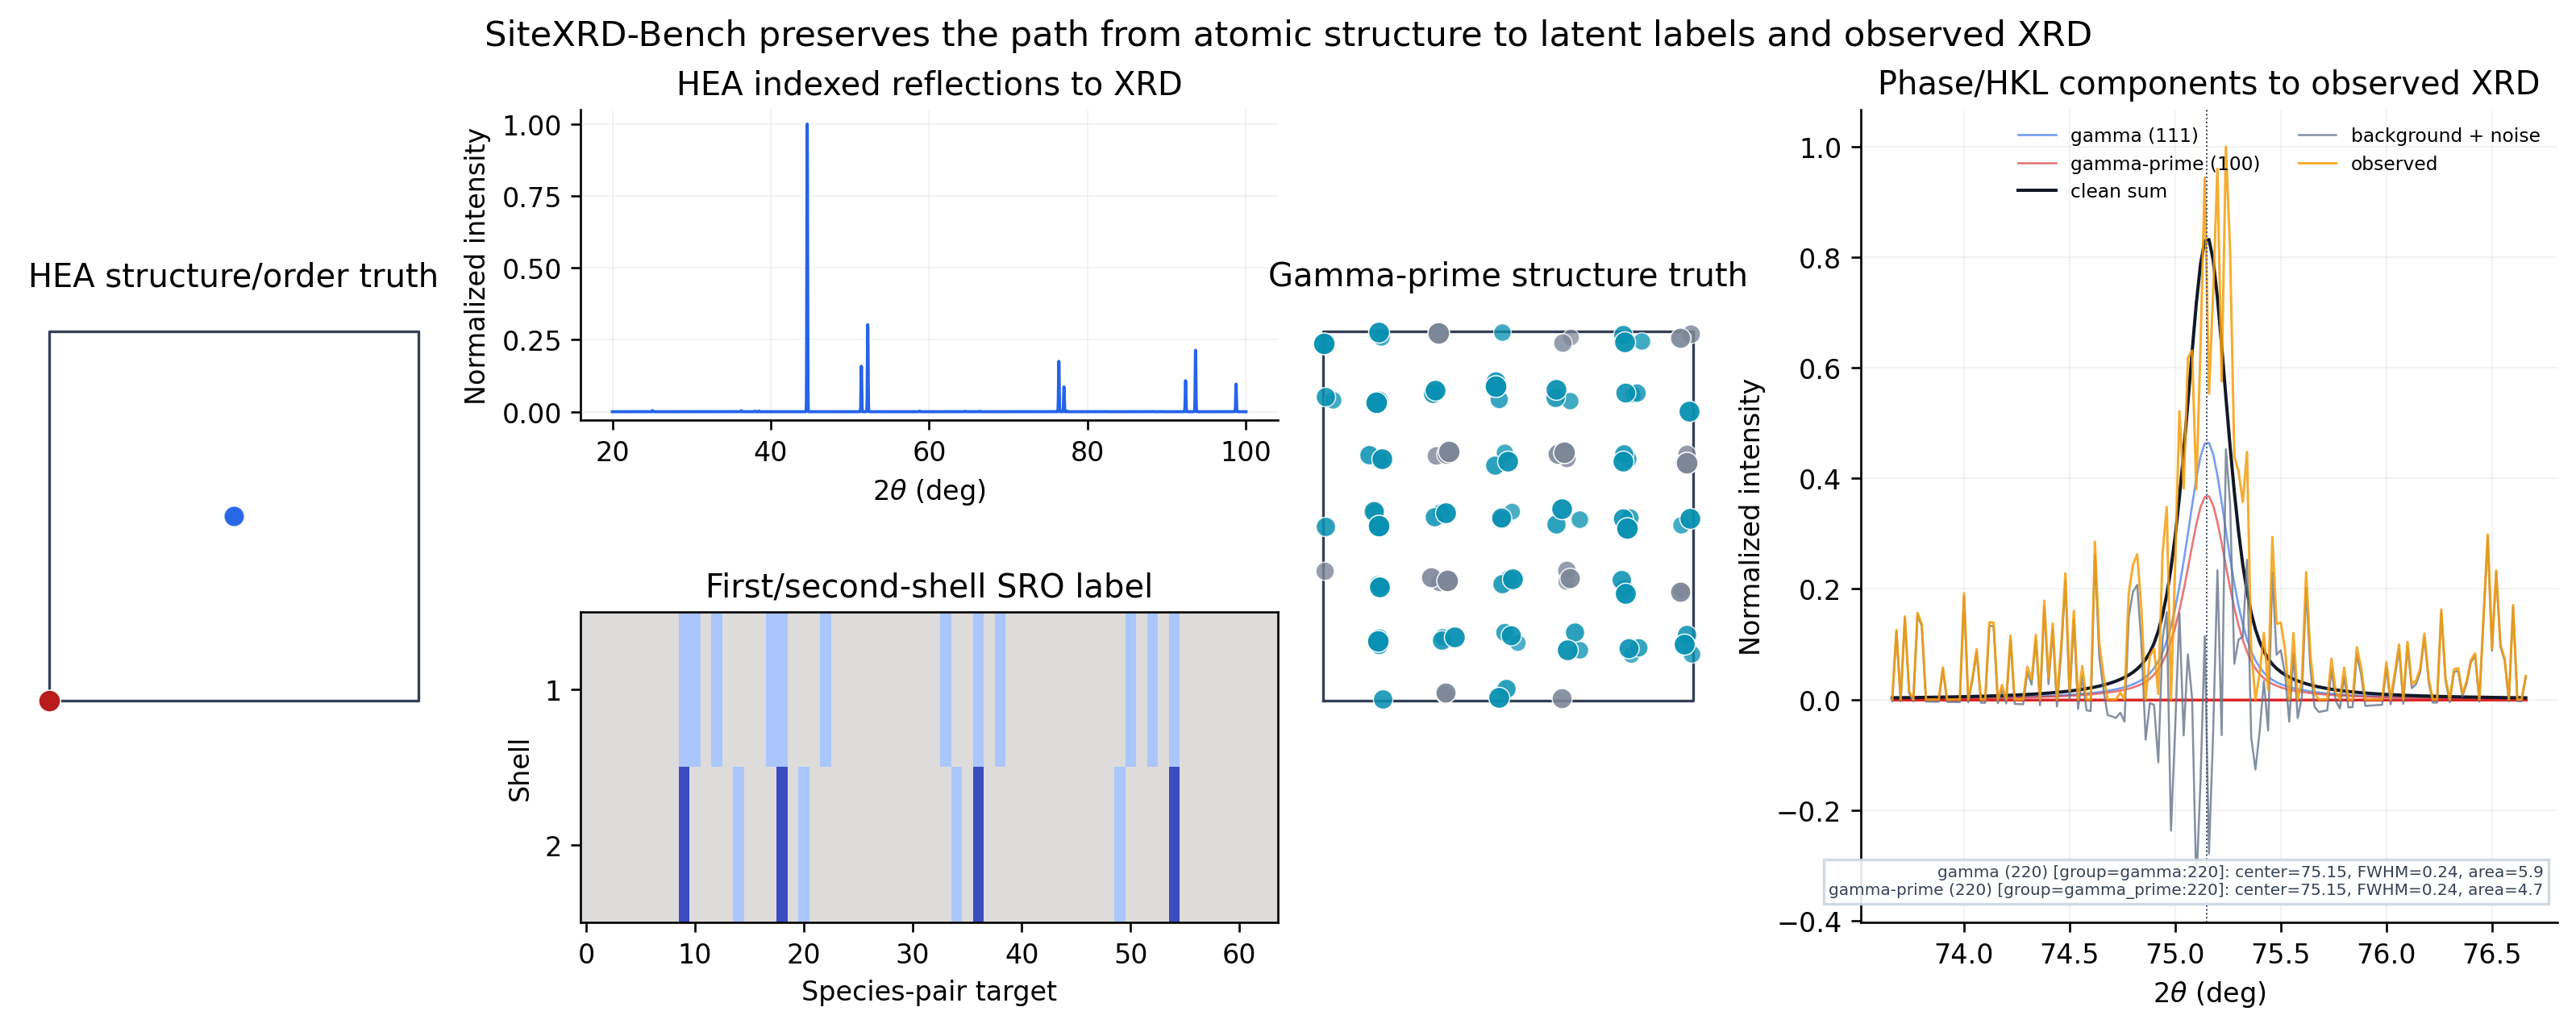
\includegraphics[width=\textwidth]{generated/dataset_overview.png}
  \caption{The two released data tracks and their traceable forward chains.
  Every displayed object comes from a public training manifest; IDs, selection
  metrics, reasons, and input hashes are stored in the visual manifest.}
  \Description{HEA and gamma/gamma-prime structures are linked to reflections,
  latent labels or component profiles, clean patterns, and observations.}
\end{figure*}}{}

\begin{table}[t]
  \caption{Representative resources and released supervision. ``Missing''
  denotes absence from that resource's contract, not a defect.}
  \label{tab:related_resources}
  \scriptsize
  \begin{tabular}{@{}p{0.19\columnwidth}p{0.27\columnwidth}p{0.44\columnwidth}@{}}
    \toprule Resource & Released evidence & Missing for this benchmark \\
    \midrule
    COD~\cite{grazulis2012cod} & Open crystal structures & Component truth and grouped inverse evaluation \\
    Materials Project~\cite{jain2013materialsproject} & Computed structures/properties & Observed-pattern component provenance \\
    RRUFF~\cite{lafuente2015rruff} & Experimental mineral XRD & SRO and phase/HKL component truth \\
    HEA source~\cite{li2024dataset} & Relaxed structures/attributes & XRD tasks, perturbations, evaluator \\
    \dataset{} & SRO, reflections, components, XRD, OOD & Exact experimental latent truth \\
    \bottomrule
  \end{tabular}
\end{table}

\section{Dataset Overview}

For latent material state $z$ and acquisition condition $n$, the release stores
\begin{equation}
z\longrightarrow\mathcal{R}(z)\longrightarrow
\{c_k(\theta;z,n)\}_{k=1}^{K}\longrightarrow y(\theta),
\end{equation}
where $\mathcal{R}$ is the indexed reflection set and $c_k$ is a broadened
phase/HKL component. The observation is
\begin{equation}
y(\theta)=\sum_{k=1}^{K}c_k(\theta;z,n)+b(\theta;n)+\epsilon(\theta;n).
\end{equation}
Stable sample, structure-state, parent-group, reflection, and component IDs link
every level to a frozen manifest, configuration, checksum, and provenance row.

Every source row receives a stable ID, canonical structure hash, composition,
quality result, and eligibility flags. Derived labels are deterministic,
versioned functions of formal structures. Rejected rows remain accounted for.
Perturbed views inherit their clean parent's group and cannot cross a split.
Thus reconstruction can be scored independently from recovery of $z$ or
$\{c_k\}$.

\section{HEA-SRO Data}

The source corpus contains ordered cells and SQS structures with up to 125 atoms
from Al, Co, Cr, Cu, Fe, Mn, Ni, and Si
~\cite{li2024dataset,li2024modeling}. Of 84,024 source rows, 84,019 pass quality
checks and five are rejected. Each accepted structure has one immutable clean
Cu K$\alpha$ pattern with 4,001 points. Perturbations are indexed as views, not
additional structures.

For species $a,b$ and shell $s$, the primary target is
\begin{equation}
\alpha_{ab}^{(s)}=1-\frac{P(b\mid a,s)}{c_b},
\end{equation}
where $c_b$ is the global concentration. Each sample stores complete masked
first/second-shell species-pair matrices, topology, shell definitions, and
provenance to the relaxed structure. Exact atom-index recovery is not a task.

\IfFileExists{generated/hea_sro_example.png}{
\begin{figure*}[t]
  \centering
  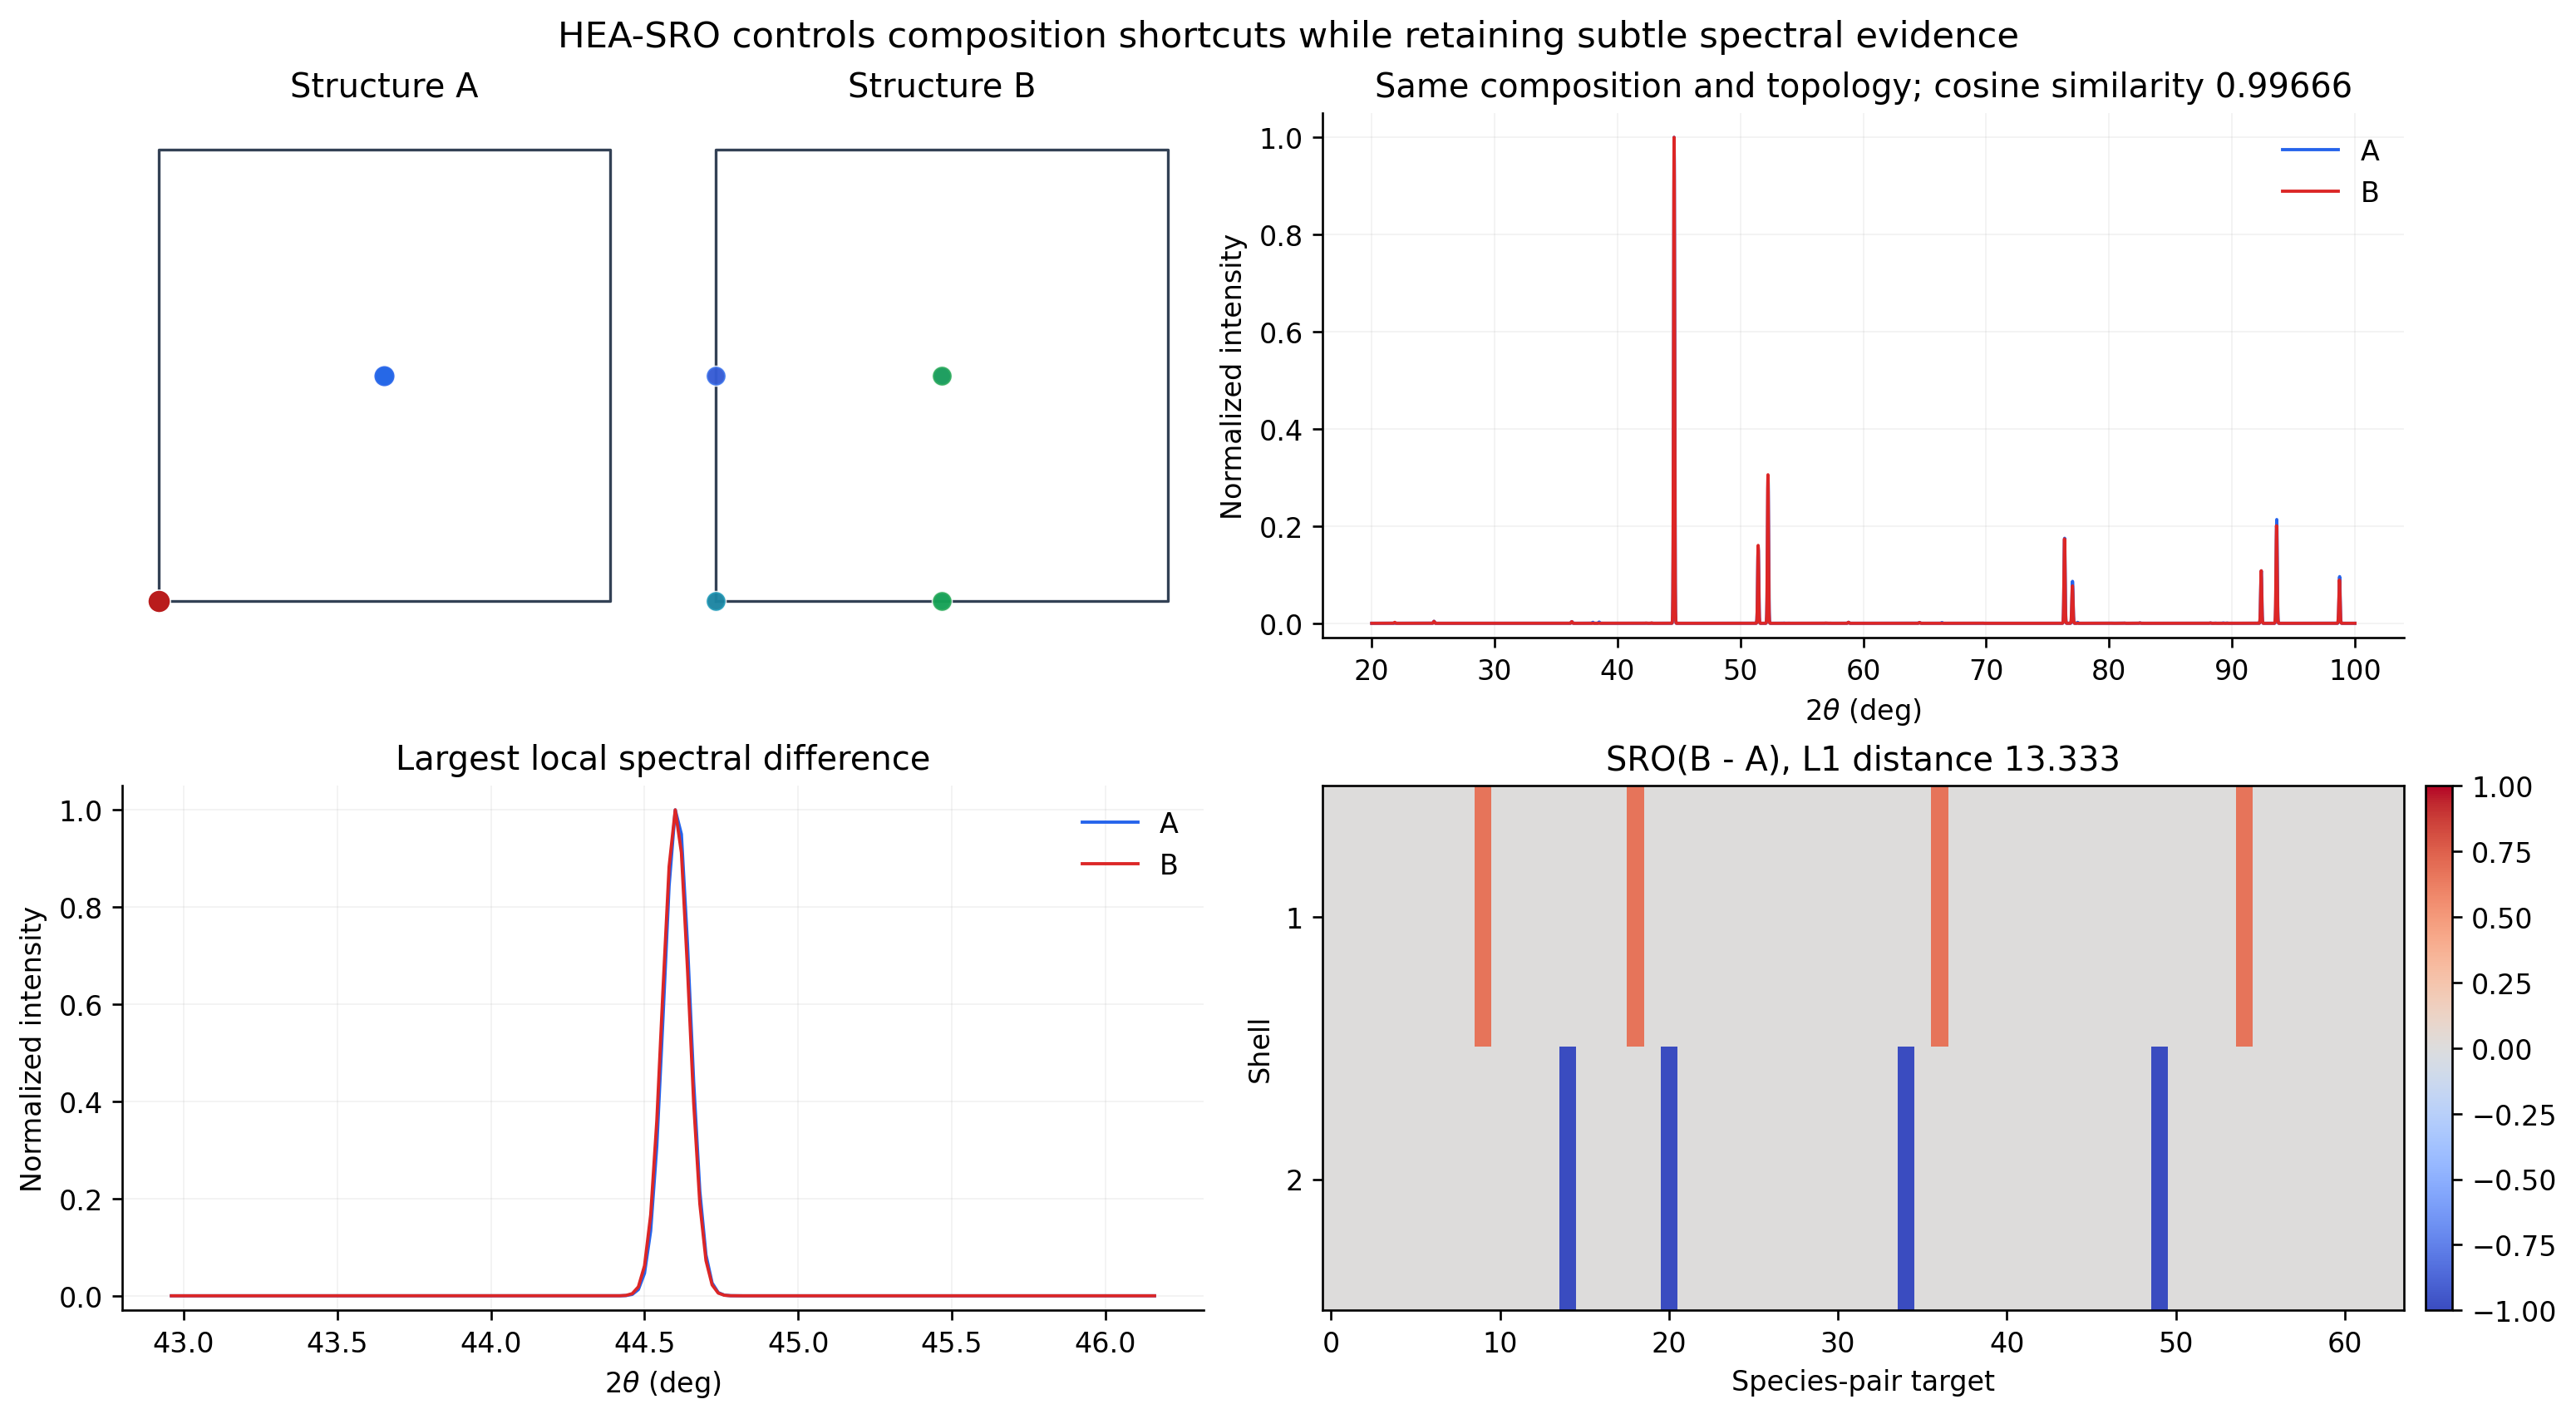
\includegraphics[width=\textwidth]{generated/hea_sro_example.png}
  \caption{Deterministically selected HEA-SRO training pair: same reduced
  composition and BCC/FCC topology, XRD cosine similarity at least 0.995, and
  maximum eligible SRO $L_1$ difference. The full spectra, most different local
  peak region, and first/second-shell SRO difference are shown.}
  \label{fig:hea_sro_example}
  \Description{Composition-matched structures have nearly identical XRD but
  different local chemical order.}
\end{figure*}}{}

Matching composition and topology blocks a composition shortcut, while the
near-identical spectra retain different local order. This is why the dataset
needs both SRO labels and identifiability analysis. Family is retained only as
an automated evidence diagnostic. A 1,000-parent counterfactual diagnostic
contains 4,000 same-composition occupancy pairs; none exceeds its
parent-specific simulated-noise floor. Ambiguous pairs are not ranking
negatives, and the threshold is not lowered to meet a quota.

\section{Gamma/Gamma-Prime Decomposition Data}

Gamma-Decomp is the stable task ID for this \gphase{}/\gp{} track. The generator
pairs FCC \gphase{} and \lone{} \gp{} structures and varies phase
weight, broadening, strain, crystallite size, background, zero shift, and noise
within declared ranges. Physically relaxed and parameterized counterfactual
pairs are explicitly distinguished. Component truth is stored before summation.

Gamma-Decomp v1.1 contains 10,000 mixtures, 21,116 windows, 175,150 raw
reflection-provenance rows, and 165,150 full-pattern scoring components. The
window view has 34,983 scoring components. Strictly coincident \gp{} $(221)$ and
$(300)$ reflections remain separate in provenance but merge into an equivalent
HKL scoring group. Seventeen phase/HKL groups are evaluated.

Overlap difficulty is quantitative and frozen in the manifest. For every pair
of components in a window, the separation ratio is
\[
\rho_{ij}=|m_i-m_j|/\{(w_i+w_j)/2\},
\]
where $m$ is peak center and $w$ is FWHM. The window difficulty uses
$\rho_{\min}=\min_{i<j}\rho_{ij}$: single if no scored pair exists, severe if
$\rho_{\min}<0.5$, strong if $0.5\le\rho_{\min}<1$, partial if
$1\le\rho_{\min}<2$, and resolved if $\rho_{\min}\ge2$. Thus ``severe
overlap'' means peak centers are separated by less than half the average FWHM,
not an aesthetic choice made after seeing model errors.

\IfFileExists{generated/gamma_decomp_example.png}{
\begin{figure*}[t]
  \centering
  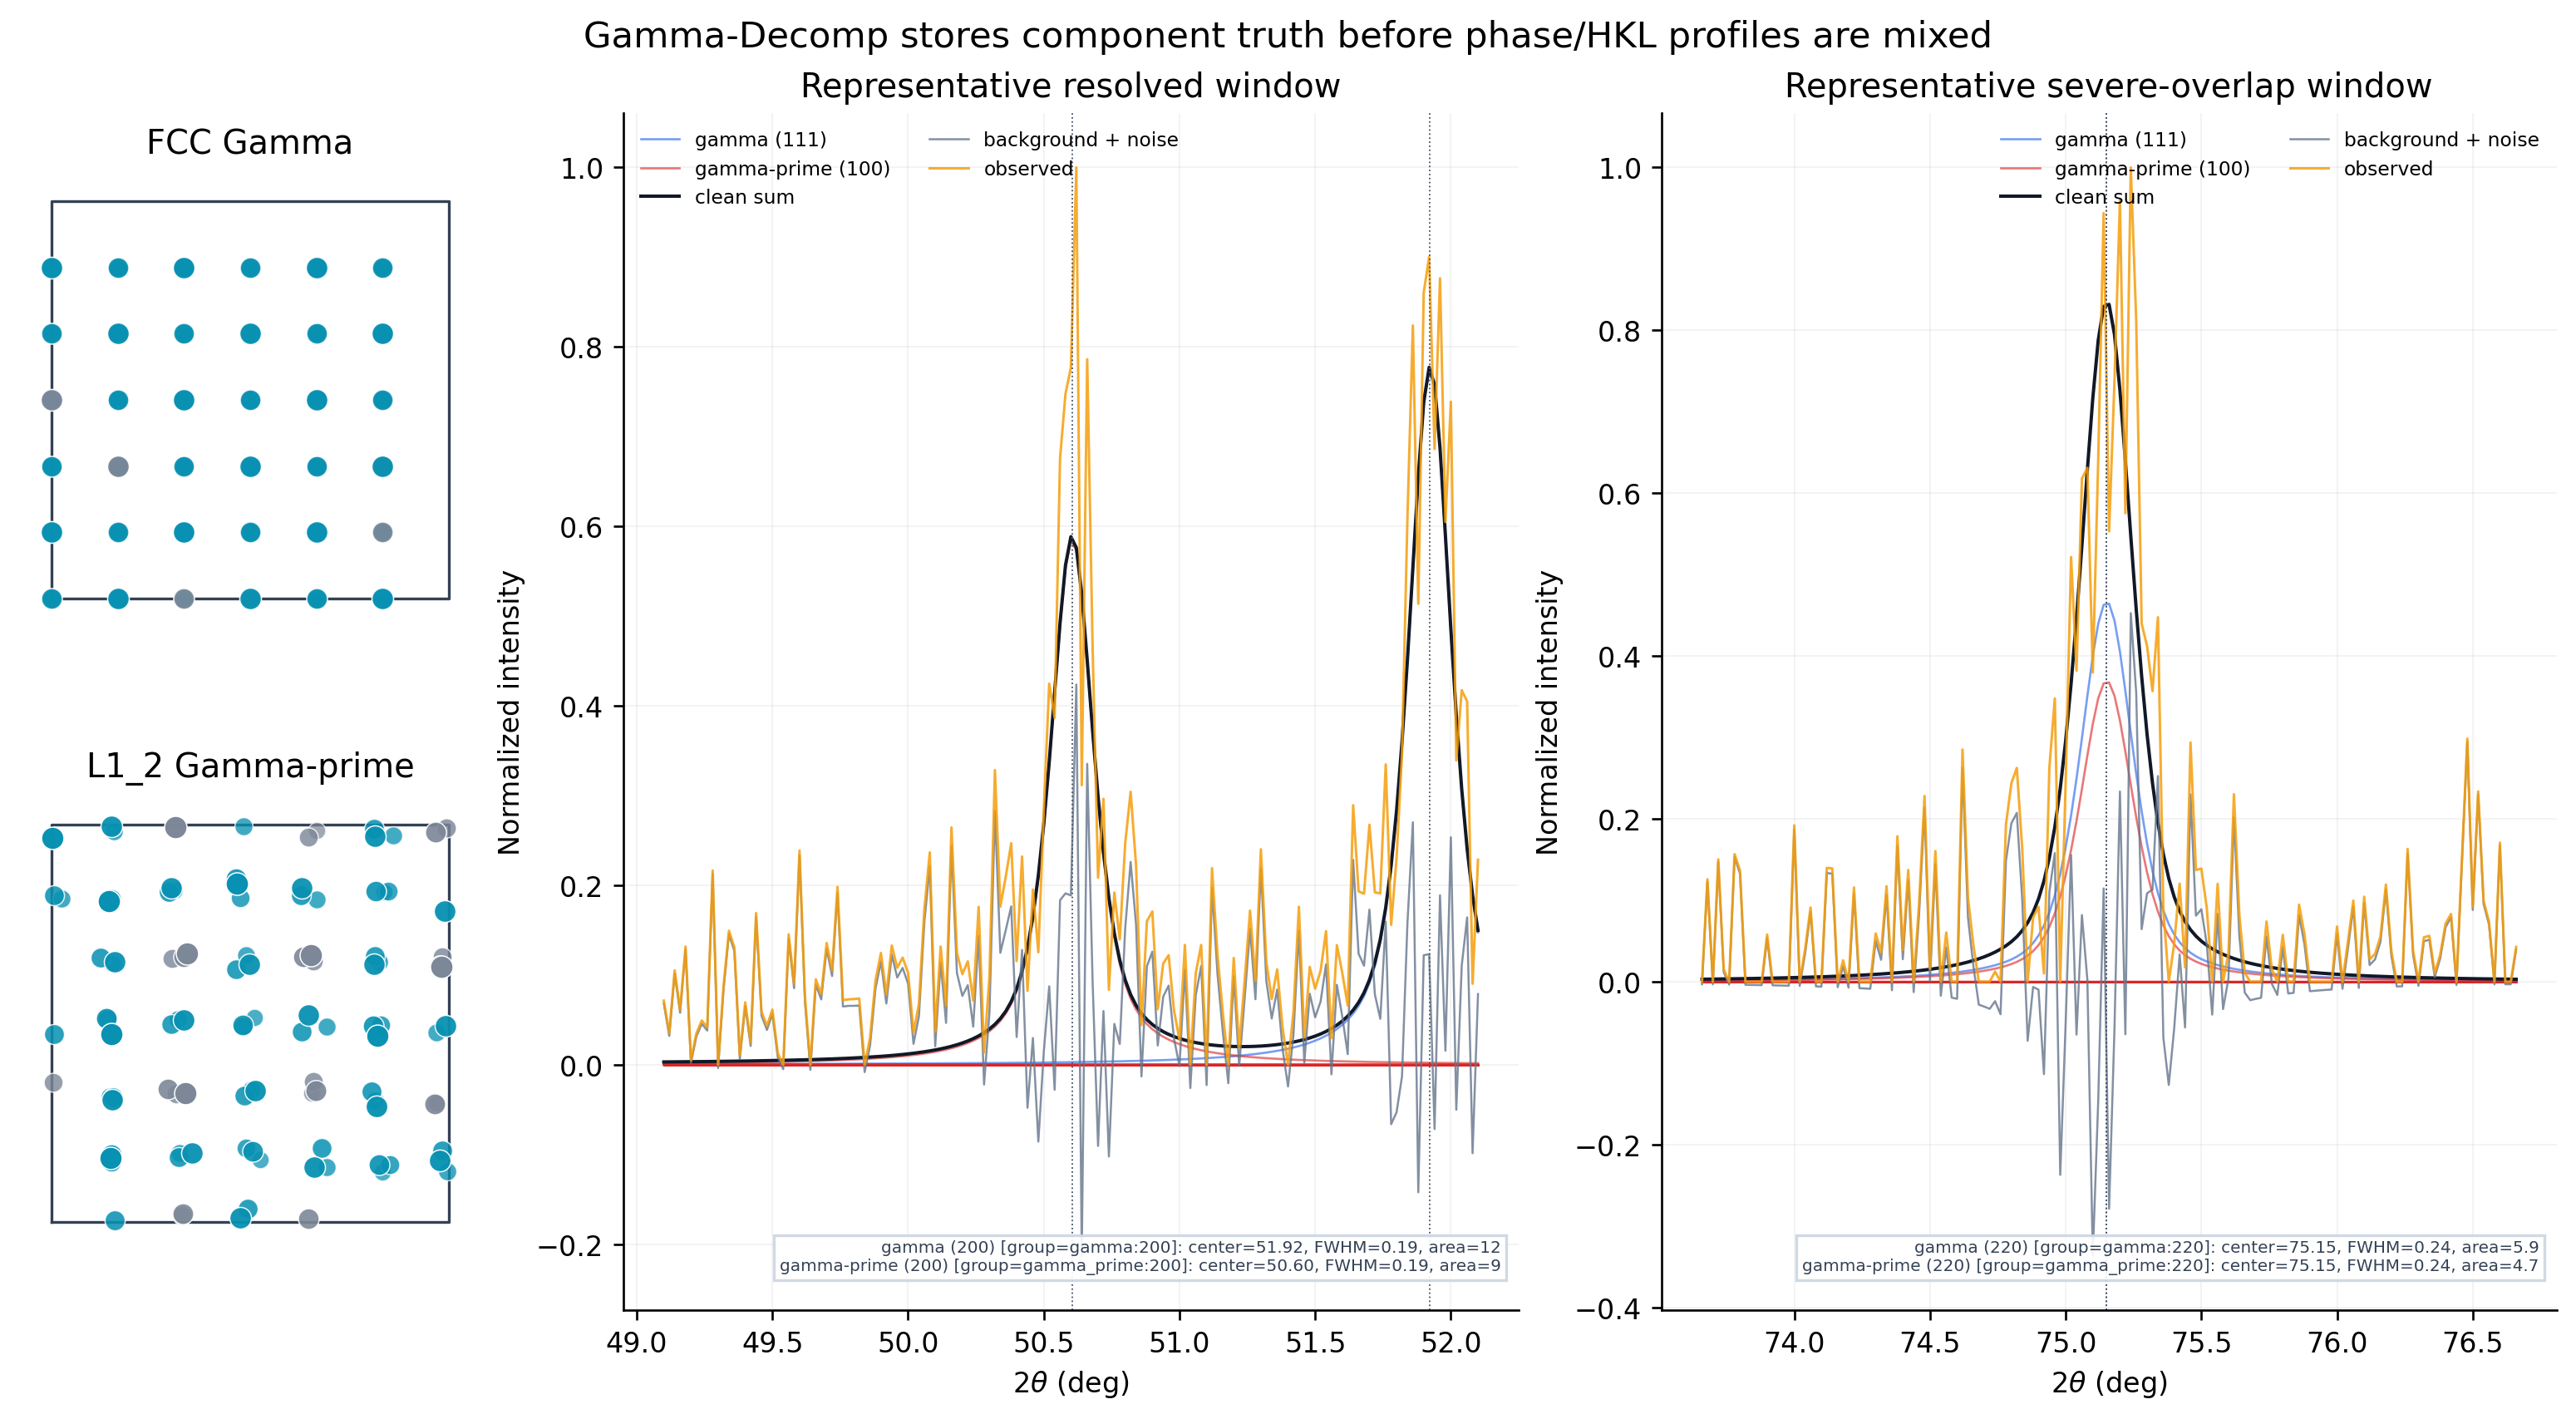
\includegraphics[width=\textwidth]{generated/gamma_decomp_example.png}
  \caption{Gamma-Decomp training examples nearest to the resolved and
  severe-overlap medians in component count, SNR, and phase weight. The panels
  show FCC \gphase{}, \lone{} \gp{}, phase/HKL profiles, clean sum,
  background/noise residual, observed pattern, center, FWHM, and area.}
  \Description{Resolved and severely overlapping windows show multiple
  physical components combining into observed peaks.}
\end{figure*}}{}

The target is an unordered component set with phase, equivalent HKL group,
center, width, area, and profile parameters. An observed peak may contain
several such components. Low reconstruction error therefore does not imply
correct latent decomposition; evaluation uses deterministic optimal bipartite
matching rather than output order.

\section{Coverage, Tasks, and Splits}

The clean reference uses Cu K$\alpha$, $20^\circ$--$100^\circ$ in $2\theta$,
and $0.02^\circ$ spacing. Reflection tables retain position, intensity, HKL,
and multiplicity. Clean truth is separated from broadening, background, strain,
texture, and noise. Validation/test perturbations are frozen.

\IfFileExists{generated/dataset_coverage.png}{
\begin{figure*}[t]
  \centering
  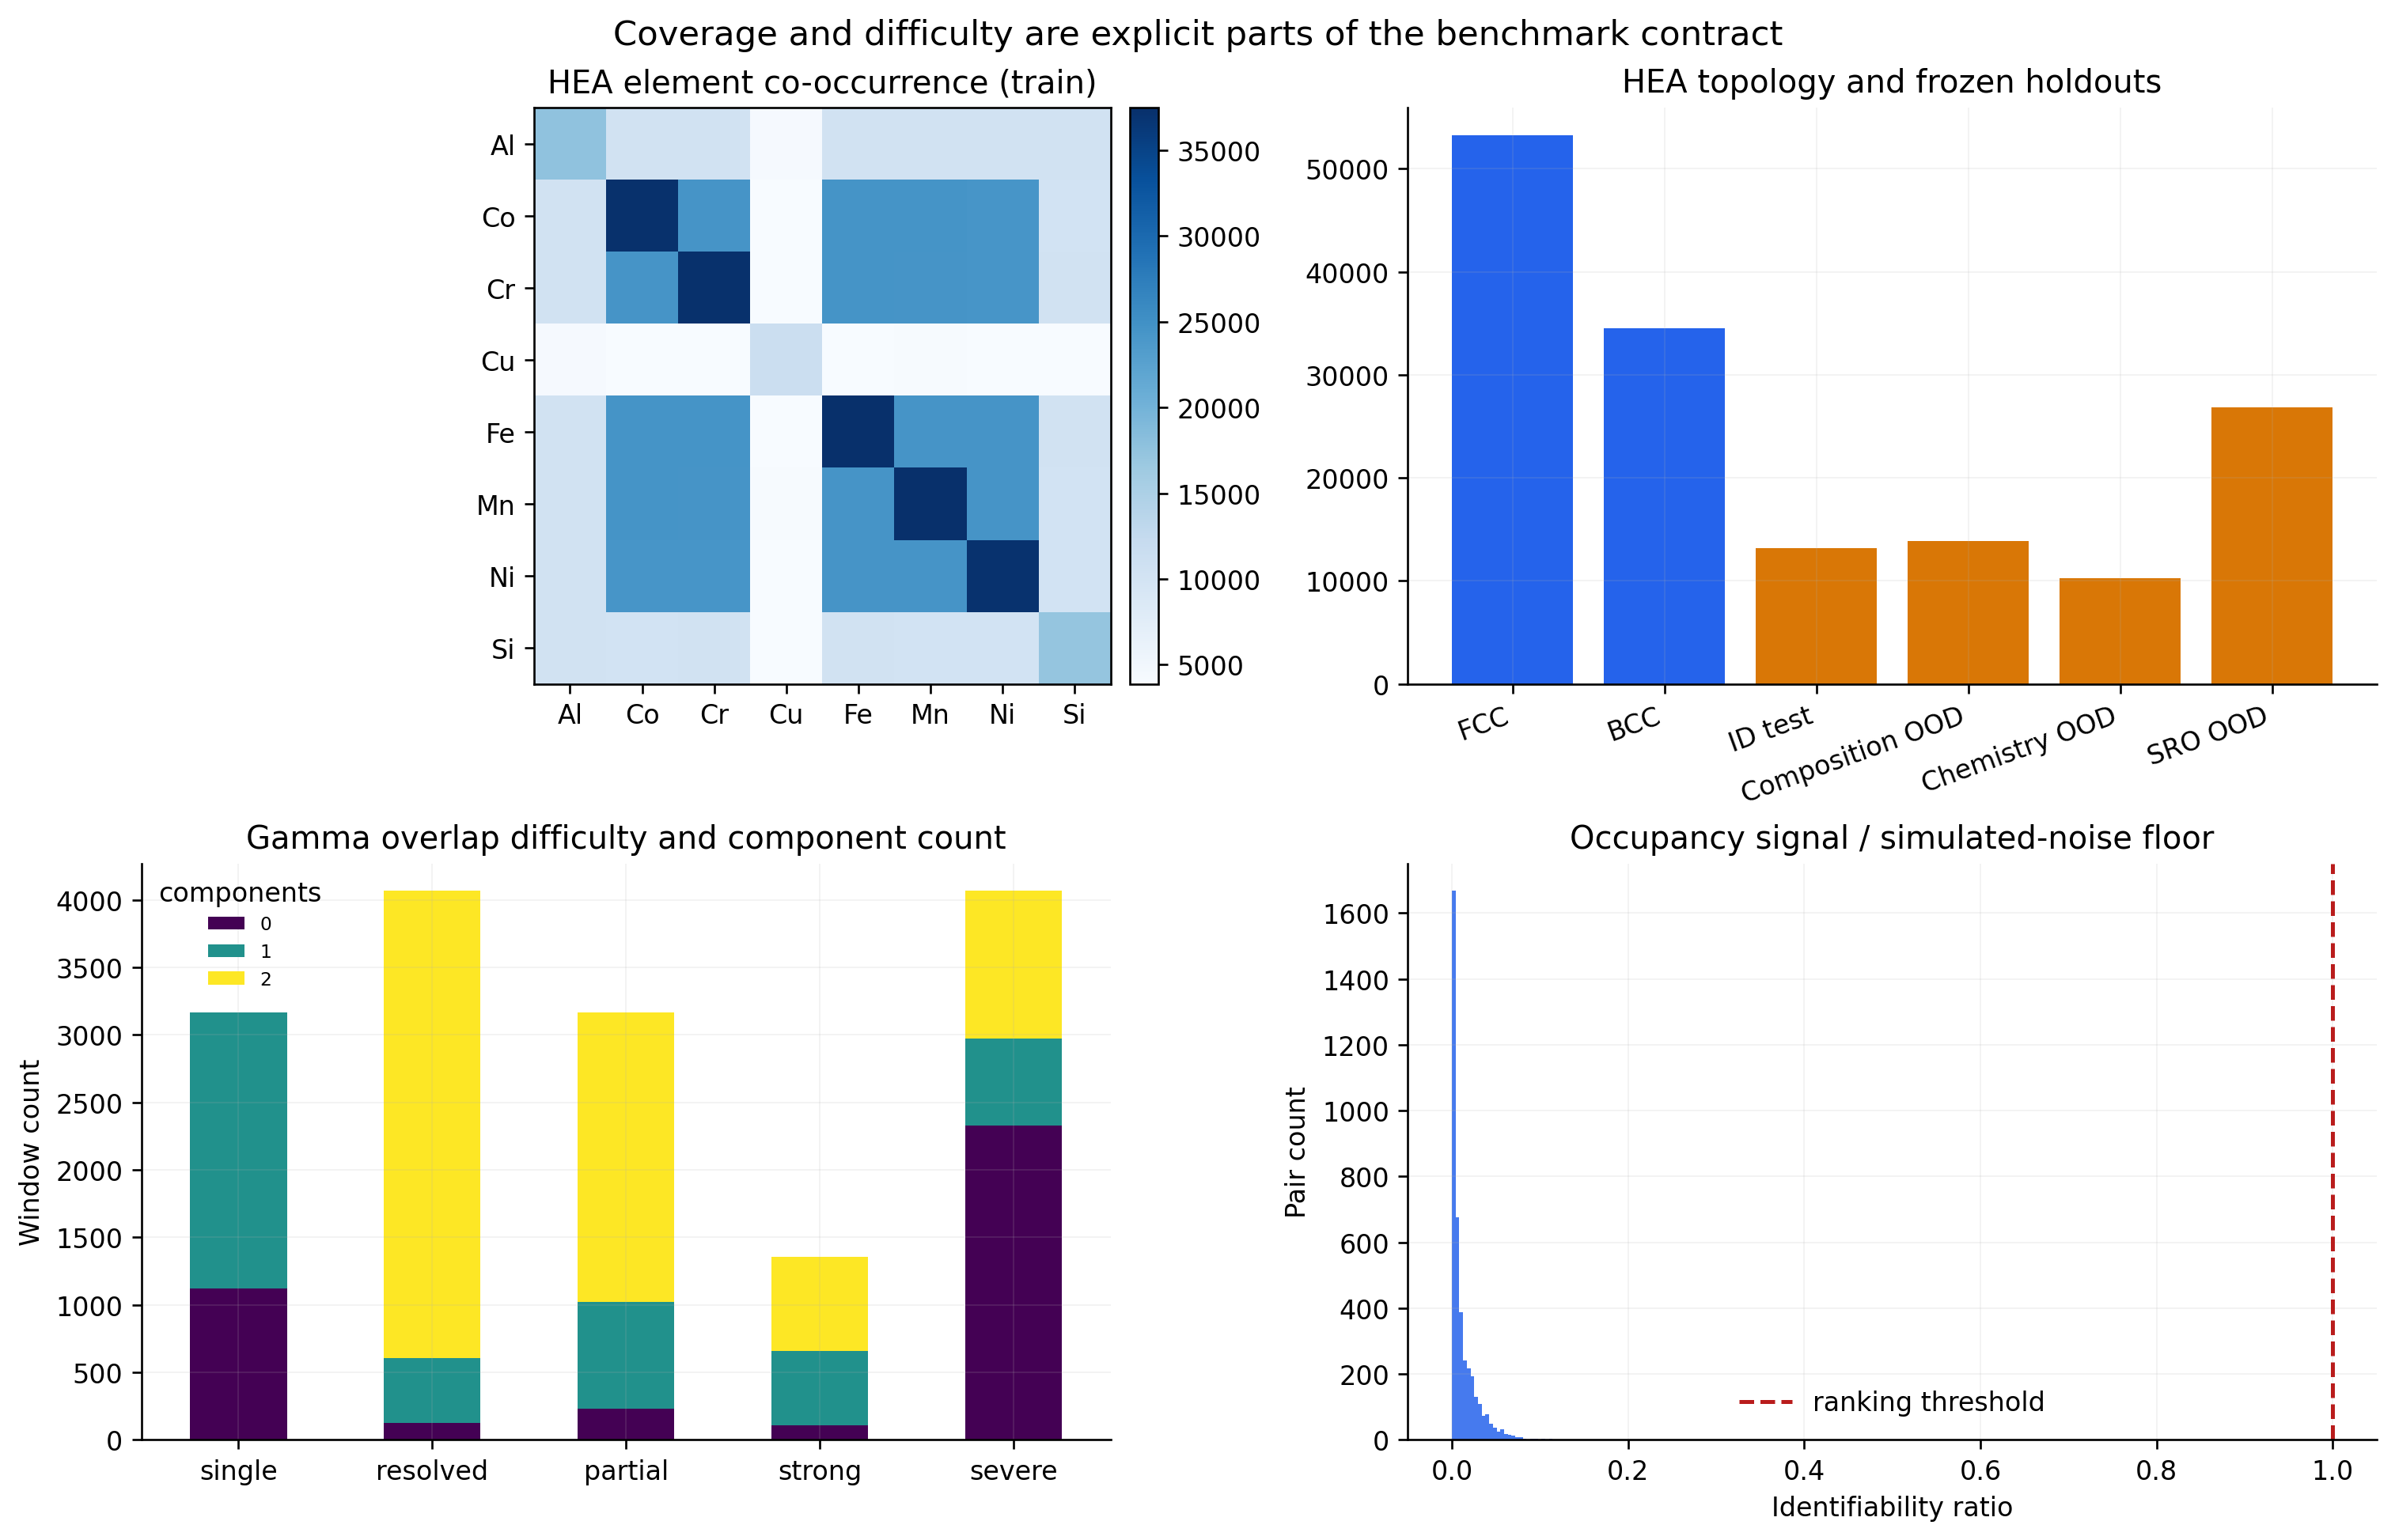
\includegraphics[width=\textwidth]{generated/dataset_coverage.png}
  \caption{Manifest-derived coverage and difficulty: HEA element
  co-occurrence, BCC/FCC and ID/OOD support, Gamma component-count/overlap
  support, and occupancy identifiability ratio with frozen threshold 1.0.}
  \Description{Four panels summarize HEA chemistry and splits, Gamma overlap
  difficulty, and occupancy signal relative to simulated noise.}
\end{figure*}}{}

\begin{table*}[t]
  \caption{Dataset and task contract. Both tracks belong to one release and
  are scored independently. Reconstruction is supplementary and never replaces
  a latent metric.}
  \label{tab:contract}
  \scriptsize\setlength{\tabcolsep}{3pt}
  \begin{tabular}{p{0.09\textwidth}p{0.13\textwidth}p{0.20\textwidth}p{0.20\textwidth}p{0.24\textwidth}}
    \toprule Track & Released scale & Target & Frozen splits & Primary metrics \\
    \midrule
    HEA-SRO & 84,019 structure--XRD pairs & Masked first/second-shell Warren--Cowley matrices & ID; composition, chemistry, SRO OOD & Parent-macro masked MAE; per-shell Spearman \\
    Gamma-Decomp & 10,000 mixtures; 21,116 windows & Unordered phase/HKL components and peak parameters & Instrument ID/OOD; resolved, partial, severe & Matched component F1; phase/HKL and count accuracy \\
    \bottomrule
  \end{tabular}
\end{table*}

HEA groups structure hashes, parents, and all observation views before assigning
ID, composition OOD, chemistry OOD, and SRO OOD splits. Gamma groups parent
pairs and views before instrument and overlap slices. Nearest-neighbor audits
cover structure and spectral spaces. An ordinary random split is not presented
as evidence of new-chemistry or acquisition generalization.

HEA macro-averages masked MAE within a parent and then across parents. Relative
improvement over mandatory Composition Ridge is
\begin{equation}
S_{\mathrm{SRO}}=100\max(0,1-\mathrm{MAE}_{model}/\mathrm{MAE}_{base}).
\end{equation}
Gamma reports component F1, phase/HKL and count accuracy, and errors in center,
width, area, and profile. Whole-pattern error remains supplementary. Random-seed
standard deviations and 2,000-replicate paired-parent bootstrap intervals (seed
2027) are reported separately. No cross-track composite score is defined
because SRO matrix regression and unordered component recovery have different
target spaces and metrics.

\section{Benchmark Validation}

The formal HEA matrix consists of Composition Ridge, Peak XGBoost, ResNet1D, and Spectrum Transformer.
Ridge is deterministic; the three XRD models use
split-specific training memberships and seeds 2027--2031. A
physics-constrained HEA experiment is appendix-only and is not part of the
formal four-model matrix. Gamma adds a no-spectrum prior, constrained
pseudo-Voigt fit, peak features, neural set predictors, and a
physics-constrained component model.

The physics-constrained variants are reported but not promoted into the primary
leaderboard for two reasons. First, they introduce additional forward-profile
structure and latent peak-parameter priors, so they test a different contract
than end-to-end learning from the released inputs. Second, their gains are not
uniform: in HEA-SRO the appendix variant changes MAE by only
0.0011--0.0024 relative to Spectrum Transformer, while in Gamma-Decomp it is
competitive on full patterns but much weaker on fixed overlap windows. Keeping
them in the appendix makes the design choice explicit without letting a
specialized prior define the benchmark's main comparison.

On HEA ID, Spectrum Transformer reduces parent-macro MAE from 0.4496 to 0.3400.
The 24.4\% reduction has a parent-bootstrap interval of 23.8--24.9\% over 12,556
groups. Peak XGBoost is competitive; ResNet1D does not consistently beat the
metadata control, demonstrating why a simple shortcut baseline is necessary.

On Gamma test data, Peak Feature attains component F1 of 0.683 on full patterns
and 0.809 on windows, versus 0.421 and 0.072 for the no-spectrum prior. For seed
2027, paired-parent improvements are 0.260 (0.207--0.313) and 0.740
(0.717--0.762). Neural predictors are not uniformly superior: the Gamma
physics-constrained model scores 0.627 on full patterns but 0.304 on windows.
The occupancy diagnostic remains a formal negative result: 0/4,000 pairs exceed
the frozen ratio 1.0.

\begin{table*}[t]
  \centering
  \caption{Compact primary results. HEA reports parent-macro SRO MAE for ID and
  three OOD splits; Gamma reports component F1 for full patterns and windows.
  SD is across declared seeds; ``--'' means not applicable.}
  \label{tab:primary_results}
  % Generated by alloy_xrd_bench.dataset_paper_visuals; do not edit.
\begin{minipage}[t]{0.48\textwidth}
\centering\scriptsize\setlength{\tabcolsep}{3pt}
\textbf{HEA-SRO parent-macro MAE}\par\smallskip
\begin{tabular}{llrr}
\toprule Split & Model & MAE $\downarrow$ & SD \\
\midrule
chemistry\_ood & Composition Ridge & 0.4340 & 0.0000 \\
chemistry\_ood & Peak XGBoost & \underline{0.3575} & 0.0000 \\
chemistry\_ood & ResNet1D & 0.4396 & 0.0055 \\
chemistry\_ood & \textbf{Spectrum Transformer} & \textbf{0.3362} & 0.0035 \\
composition\_ood & Composition Ridge & 0.4433 & 0.0000 \\
composition\_ood & Peak XGBoost & \underline{0.3621} & 0.0000 \\
composition\_ood & ResNet1D & 0.4632 & 0.0164 \\
composition\_ood & \textbf{Spectrum Transformer} & \textbf{0.3402} & 0.0022 \\
id & Composition Ridge & 0.4496 & 0.0000 \\
id & Peak XGBoost & \underline{0.3621} & 0.0000 \\
id & ResNet1D & 0.4414 & 0.0202 \\
id & \textbf{Spectrum Transformer} & \textbf{0.3400} & 0.0009 \\
sro\_ood & Composition Ridge & 0.5142 & 0.0000 \\
sro\_ood & Peak XGBoost & \underline{0.4493} & 0.0000 \\
sro\_ood & ResNet1D & 0.5020 & 0.0136 \\
sro\_ood & \textbf{Spectrum Transformer} & \textbf{0.4291} & 0.0025 \\
\bottomrule
\end{tabular}
\end{minipage}\hfill
\begin{minipage}[t]{0.48\textwidth}
\centering\scriptsize\setlength{\tabcolsep}{3pt}
\textbf{Gamma-Decomp component F1}\par\smallskip
\begin{tabular}{llrr}
\toprule View & Model & F1 $\uparrow$ & SD \\
\midrule
Full & No-spectrum prior & 0.421 & -- \\
Window & No-spectrum prior & 0.072 & -- \\
Full & \textbf{Peak Feature} & \textbf{0.683} & 0.003 \\
Window & \textbf{Peak Feature} & \textbf{0.809} & 0.002 \\
Window & Pseudo-Voigt (BIC) & \underline{0.527} & -- \\
Full & ResNet Set & 0.473 & 0.015 \\
Window & ResNet Set & 0.466 & 0.114 \\
Full & Transformer Set & 0.599 & 0.163 \\
Window & Transformer Set & 0.494 & 0.038 \\
Full & Physics-constr. & \underline{0.627} & 0.155 \\
Window & Physics-constr. & 0.304 & 0.059 \\
\bottomrule
\end{tabular}
\end{minipage}

\end{table*}

All prediction IDs must match the declared split exactly. Perfect-oracle tests
attain the exact optimum, shuffled predictions degrade, and component
permutations leave set scores unchanged. Release readiness depends on complete
IDs, splits, seeds, manifests, checksums, and statistics, not on whether a model
beats Ridge.

\FloatBarrier

\section{Availability, Limitations, and Conclusion}

Code, configuration, evaluation, cards, download tools, and smoke data are
released separately from the sharded structures/XRD/labels and the frozen
metadata/checksum snapshot. The final paper records public GitHub, Hugging Face,
and Zenodo DOI links only after the records exist and anonymous HTTP checks
succeed; no provisional URL or unminted DOI is printed. The repository also
contains the Dataset Card, Benchmark Card, Croissant metadata, citation record,
and release checklist.

The computational structure is ground truth for generated samples, but does not
prove that experimental powder XRD uniquely determines occupancy. Periodic
supercells, similar scattering factors, finite resolution, texture, microstrain,
nanostructure, and unmodeled phases can make inversion ambiguous. Family labels
are automated and unadjudicated. Occupancy uses simulated perturbations only;
real repeated-measurement import and noise calibration are v1.2 gates.

The admitted HEA experimental set supports only mother-phase trends
~\cite{wang2021heaf}. The Ni-based sanity set contains licensed raw arrays for
heat-treated IN718 and AM718R, where \gp{} and gamma-double-prime superlattice
reflections are not distinguishable
~\cite{markanday2022repairdata,markanday2022repair}. It supports phase-level and
whole-pattern checks, not experimental component-level validation.

\dataset{} therefore unifies two complementary inverse problems within one
versioned benchmark: subtle local chemical order and overlapping \gphase{}/\gp{}
phase evidence. Its central claim is not that every latent variable is
recoverable, but that recoverability, shortcut use, OOD behavior, and abstention
can now be evaluated against traceable truth.

\bibliographystyle{ACM-Reference-Format}
\bibliography{sitexrd_bench_references}

\appendix

\section{Secondary Results and Diagnostics}

The physics-constrained HEA experiment is exploratory and excluded from the
formal matrix. Full per-seed results, parameter errors, instrument/overlap
slices, and perturbation curves remain in machine-readable evidence. The PDF
keeps the main four data figures in the body; secondary model-slice plots are
released with the generated artifacts to preserve the page budget:
\path{generated/hea_occupancy_signal_noise.png},
\path{generated/hea_perturbation_severity.png},
\path{generated/gamma_instrument_slices.png}, and
\path{generated/gamma_overlap_difficulty.png}. Detailed generated tables remain
in \path{generated/hea_sro_results.tex} and
\path{generated/gamma_decomp_results.tex}.

\subsection{Diagnostic Slices}

The occupancy panel places every controlled pair below its parent-specific
simulated-noise threshold, supporting abstention rather than forced ranking.
The perturbation curve measures a different failure mode: SRO remains a defined
structure-derived target even when observation quality degrades. For Gamma,
instrument shift changes component F1 much less than severe overlap. Reporting
these axes separately prevents a single average from hiding whether failure is
caused by observability, acquisition shift, or component coincidence.

\subsection{Extended HEA-SRO Results}

Across all four HEA splits, Spectrum Transformer is the strongest member of the
formal model matrix. The exploratory physics-constrained variant changes MAE by
only 0.0011--0.0024 relative to Spectrum Transformer, whereas ResNet1D can fall
behind the composition-only control under composition and SRO shift. These
small gains are why the physics-constrained variant is not promoted into the
formal comparison.

\subsection{Extended Gamma-Decomp Results}

Peak Feature gives the strongest component F1 on both views and the strongest
window count accuracy. The neural set predictors are less stable across seeds,
and the physics-constrained model does not recover its full-pattern advantage
on windows. Center, width, and area errors are therefore reported separately
from component F1 rather than collapsed into a reconstruction-weighted score.

\end{document}
